\chapter{ Самир Михаиль, каирский феникс}
\begin{remark}
	Дисклеймер: все цитаты в данной статье приведены «as is» в соответствии с источниками, указанными в конце статьи, и по возможности верифицированы с израильскими данными. Автор не гарантирует, что все события развивались именно так, как их описывает главный герой данной статьи, при этом автор приложил все усилия для того, чтобы найти подтверждения его словами с противоположной стороны. Конкретные источники тех или иных цитат могут быть приведены при необходимости.
\end{remark}
\section{Об арабских лётчиках}
Так исторически сложилось, что действия арабов в арабо-израильских войнах принято описывать с некоторой насмешкой и иронией. С одной стороны, после 67-го года они, безусловно, заслужили такое к себе отношение. С другой - годы снисхождений стоили израильтянам нескольких страшных дней в октябре 73-го года - когда арабы смыли позор Шестидневной войны и доказали, что они тоже чего-то стоят.

Мы слышали многое об израильских пилотах - самом результативном “сверхзвуковом” (или вообще реактивном) летчике - Гиоре Эпштейне, о Йифтахе Спекторе, Амире Нахуми, и других. Имена же их оппонентов практически неизвестны за пределами арабских стран и небольшого исторического сообщества. Вряд-ли много кто слышал о Файезе Мансуре, Самире Михаиле, Мохаммеде Мусе, и других. И да, это были отличные лётчики, не хуже многих израильских. Может, их реальные успехи не так впечатляют, как, например, успехи вьетнамцев - но так и воевали они далеко не с американским строем "Тандерчифов" - а с куда более хитрым и непредсказуемым врагом.

Конечно, талантливых пилотов в Египте было меньше, чем в Израиле - но они были! Почему о них известно так мало? Отчасти, виноват арабский официоз - они тщательно скрывали и мифологизировали всё, что касается войн с Израилем. «Еврейское телеграфное агенство» придумало отличный термин — «папирусные победы». В итоге, даже самый непредвзятый арабский взгляд на события 67-82 годов невольно наводит на одну простую мысль- это правда или опять арабская параллельная вселенная, полная "папирусных" побед?

К тому-же негибкая социальная структура армии, выросшая из архаичной социальной структуры самого арабского общества, практически не давала шансов многим по-настоящему талантливым людям проявить себя. Огромное количество израильских летчиков вышло из киббуцников (по-сути, из крестьян) - Гиора Эпштейн, Моше Эртц, Коби Рихтер, и это только из очень известных. Фактически, около 30\% лётного состава в те годы были киббуцниками. Да, эти люди не перестали быть в чем-то крестьянами, но летать от этого они хуже не стали. В Египте у них не было бы ни единого шанса не то что подняться в небо, а просто оказаться рядом с самолетом. В авиацию приходили люди из достаточно обеспеченных слоев общества - просто потому, что они обладали хоть каким-то стоящим образованием. И у большинства из них не было и десятой доли той мотивации, какая была у их противников с другой стороны Суэцкого канала.

Для израильтянина быть лётчиком, пройти сложнейший отбор - большое личное достижение. Для араба - это лишь подтверждение высокого социального статуса от рождения. Отсюда - завышенная болезненная самооценка и недостаток мотивации.

Впрочем, так получалось не со всеми.

\section{Самир Азиз, лейтенант и христианин}

Самир Азиз Михаиль родился 1943-м году в семье инженера ВВС, араба-копта. Отец был категорически против того, чтобы сын стал летчиком, так что Самиру пришлось поступать в колледж ВВС практически тайно, когда отец был в командировке. Семья не принадлежала к «высшему обществу», но жила в определенном достатке, и могла позволить детям неплохое образование. И как следствие — попадание в авиацию.

Дальнейшая его судьба типична для многих молодых египетских пилотов. Выпустившись в 63-м году, начинал на МиГ-17, достаточно быстро попал на МиГ-21, которые Союз только начал поставлять египтянам. Тут с ним случился первый казус - учебные “спарки” пришли далеко не сразу, и летать приходилось сразу “соло” - пилоты отрабатывали взлет и заход на посадку на МиГ-17, “имитируя” 21-е, и только потом проделывали всё то - же самое на самом 21-м. Сумасшедшая посадочная скорость 21-го, его ускорение и мощь производили на таких “курсантов” неизгладимое впечатление - правда, пережили его не все. Справедливости ради, у израильтян спарки “Миражей” появились тоже только в 67-м году, так что это была общая проблема.

\begin{figure}[h!tb] 
	\centering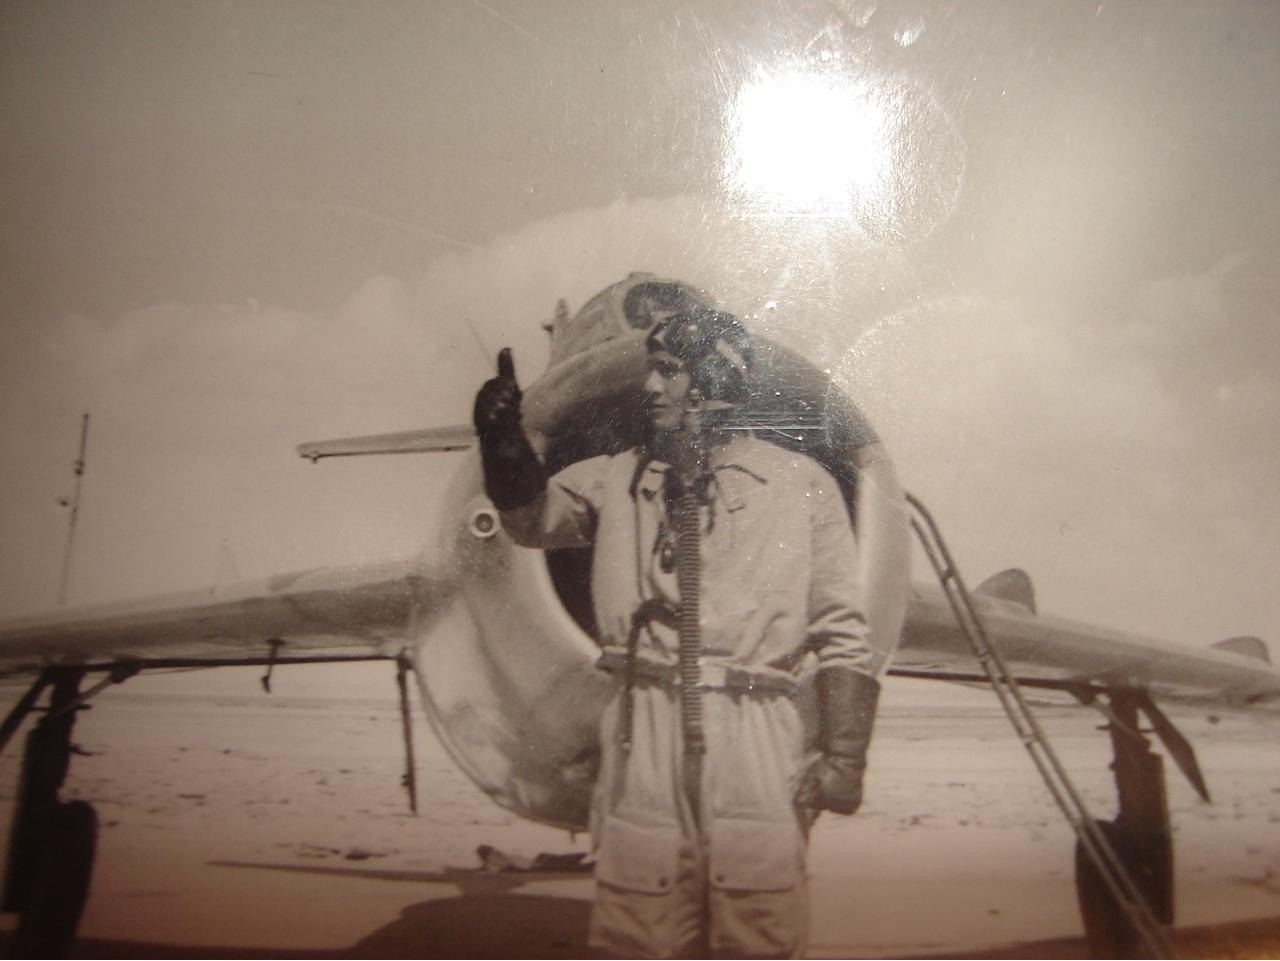
\includegraphics[scale=0.35]{History_Fenix/uRqdQTV9U2I.jpg}
	%	\label{fig:scipion} % Unique label used for referencing the figure in-text\end{document}
	%	%\addcontentsline{toc}{figure}{Figure \ref{fig:placeholder}} % Uncomment to add the figure to the table of contents%----------------------------------------------------------------------------------------
	\caption{Самир Михаиль сразу после окончания лётного курса, на фоне МиГ-17, 1963-64 год. Фото group73historians}%	CHAPTER 2
\end{figure}

В 65-м наш герой в звании лейтенанта оказался в Йемене. Что характерно, полноценных “боевых” вылетов там не было - основной задачей египтян было летать над головами местных аборигенов низЭнько-низЭнько, дабы вселить в их сердца страх и почтение к представителям высокоразвитой египетской цивилизации. Именно там Самир развил и отточил умение летать буквально по верхушкам деревьев - чем и прославился в дальнейшем. Пальмы в тех краях, надо сказать, невысокие - так что зрелище для неподготовленного зрителя получалось то ещё. Через три месяца таких полётов, египтяне вернулись домой.

Тогда же у него проявилась другая черта, свойственная скорее людям с другой стороны границы. Любопытство. В одном из вылетов до шестидневной войны, он оказался над Синаем, и, по его словам, внезапно понял, что видит Израиль почти ЦЕЛИКОМ, до Ливана. Испытываемые в тот момент чувства он описывал как очень странные - молодые египетские офицеры практически ничего не знали о евреях (кроме того, что они враги и в них надо стрелять), и ему по его словам просто было любопытно - кто эти люди?!

Блицкриг Шестидневной войны Самир, как и большинство египетских пилотов, встретил в гордо поднятой вверх головой - наблюдая за тем, как волна за волной, серебристые “Миражи”, “Вотуры” и “Самбады” превращают египетские аэродромы в горящие руины, а самолеты - в груды обломков. 

\begin{figure}[h!tb] 
	\centering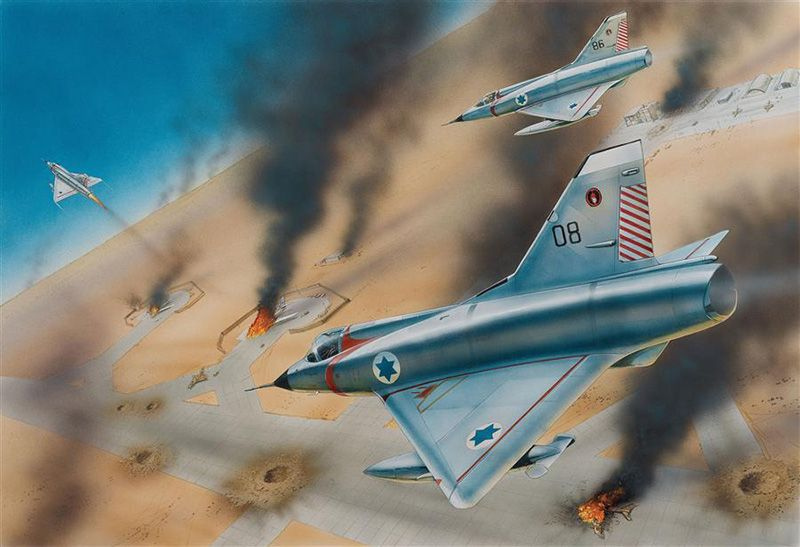
\includegraphics[scale=0.5]{History_Fenix/G0ZHOpHX9To.jpg}
	%	\label{fig:scipion} % Unique label used for referencing the figure in-text\end{document}
	%	%\addcontentsline{toc}{figure}{Figure \ref{fig:placeholder}} % Uncomment to add the figure to the table of contents%----------------------------------------------------------------------------------------
	\caption{101-я эскадрилья штурмует египетский аэродром}%	CHAPTER 2
\end{figure}

Но ВВС Египта не умерли. При помощи советских поставок, они словно птица Феникс, возродились из пепла пожаров - более того, очень быстро число современных самолетов в Египте превысило довоенное. Тогда же началась история 104-й бригады, и её наиболее успешного подразделения — 46-й эскадрильи.

В общем, уже опытный летчик Самир Азиз попал в 44-ю, а затем в 46-ю эскадрилью только что созданной 104-й истребительной авиабригады ВВС Египта. Что удивительно, при создании эскадрилья была чисто «разведывательной», и некоторое время функционировала в таком качестве. Но приблизительно к середине 1968 она превратилась в полноценную истребительную.

Самиру повезло и в другом — после того, как СССР восполнил потери Шестидневной войны, в Египте случился жесточайший дефицит подготовленных пилотов. С приблизительно 400 боевых самолётов и вертолётов, парк машин ВВС планировали расширить до 600 только истребительной и истребительно-бомбардировочной авиации, плюс порядка 300 других самолётов и вертолётов. Эти планы никогда так и не были выполнены, но и в «сокращенной» версии проблем хватало. Из 224 пилотов, квалифицированных к полётам на МиГ-17, 19, 21 и Су-7, в шестидневную войну погибло 33, и ещё около дюжины погибли или попали в плен в послевоенных столкновениях и учебных полётах в 1967 году. Карьера Самира Азиза резко пошла в гору — он был хорошим, квалифицированным, и что более важно — живым .

Надо сказать, ему очень повезло — 104-я авиабригада одной из первых получила новые МиГ-21, и в ней выросло некоторое количество очень талантливых пилотов. Сами египтяне достаточно сложно относились к новым самолётам. С одной стороны, они были существенно быстрее и манёвреннее. С другой стороны, отсутствие пушки (особенно на поздних версиях, начиная с ФЛ и до МФ) и малый запас топлива создавали проблемы. Другой сложностью были подвесные контейнеры для аэрофотосъёмки, которые они считали на столько бесполезными, что заменяли их на … камеры, снятые с ИЛ-28 Р, помещённые в 490 литровый подвесной топливный бак. Впрочем, очень скоро вылеты на фотосъёмку израильских позиций для 46-й эскадрильи ушли на второй план.

Потому что Насер начал войну на истощение. И завертелось.

\section{Первая кровь}

В то время египетские ВВС решали три основных типа задач - нанесение ударов по территории Израиля, недопущение атак израильских ВВС на позиции армии на западном берегу и аэрофотосъёмку. И то, и другое получалось так себе - налеты на позиции ЦАХАЛ всегда были сопряжены с большим риском, а эффективно перехватывать израильтян египетские пилоты долгое время просто не успевали - к тому моменту, когда перехватчики поднимались в воздух, цель уже была над Синаем. Египтяне попробовали было использовать дежурные пары, находящиеся в воздухе, но они при встрече с “Миражами” нередко очень быстро гибли.

Первый раз Самир Азиз столкнулся с израильскими летчиками 14 апреля 1979 года - когда четверка МиГ-21 вылетела на сопровождение пары Су-7 фоторазведки в районе перевала Митла. Разумеется, израильтяне тут же отправили им навстречу с авиабазы Рефидим пару “Миражей” 119-й эскадрильи (летчики Реувен Розен и Менахем Эяль), вооруженных только что полученными от американцев “Сайдвиндерами” B (“Баркан” по израильской классификации).

Египтяне тут же разумно отозвали разведчиков за канал, оставив истребители прикрывать их отход. Тут же, обе стороны подняли усиление - четверку МиГ-21 Ф-13 102-й авиабригады с авиабазы Иншас и четверку “Миражей” 119-й эскадрильи из Рефидим.

Сам Самир Азиз описывал этот бой так:

\begin{textcitation}
	“... Су-7 спикировали, чтобы произвести съёмку, а мы остались выше. Потом наземный контроль сказал - противник в 2 километрах позади меня. Мои колени задрожали — мне впервые было так страшно. Я подумал, что если меня собьют над Синаем, то я окажусь в плену. Тогда я сказал себе - “началось” - и сделал крутой вираж влево с большой перегрузкой. В этот момент ракета взорвалась рядом с самолетом Исмаила (Исмаил Хассан Имам, его ведомый). Он сказал, что его самолет поврежден - я ответил ему, чтобы он уходил за канал и приземлялся в любом подходящем месте. Я посмотрел назад и увидел пару “Миражей” за собой. Я ушел вправо с набором высоты - но они преследовали меня … Я увидел под собой Канал - и четверку МиГ-21 Ф-13, отправленную к нам на помощь. Они столкнулись с подошедшей к израильтянам четверкой “Миражей”. Я набрал высоту и скорость, огляделся, и увидел внизу МиГ-21, который преследовал “Мираж”, за которым летел другой Миг. Тогда я сказал себе - “почему бы не попробовать его сбить”? Я спикировал к одному из них, но “Мираж” быстро изменил направление. Тогда я снова набрал высоту, увидел самолёт, уходящий на восток, в сторону Израиля, спикировал к нему, выпустил ракету и увидел взрыв, а затем “Мираж” с черным дымом ушел вниз. Я не нашел вторую ракету и понял, что в первый раз выпустил их обе. Я обернулся, чтобы убедиться, что меня никто не преследует - но позади никого не было. Я видел, как “Миражи” возвращаются назад, и начал уходить за канал, чтобы они не сбили меня по пути домой. Я вернулся домой и рассказал всем, как я сбил «Мираж»”.
\end{textcitation}

В итоге, “Мираж”, за штурвалом которого был ведущий первой израильской пары Реувен Розен, сумел дотянуть до Рефидим и совершить аварийную посадку - по счастливой случайности, ни одна из жизненно важных систем не получила фатальных повреждений, хотя в самолёте насчитали больше 200 новых отверстий.

\begin{figure}[h!tb] 
	\centering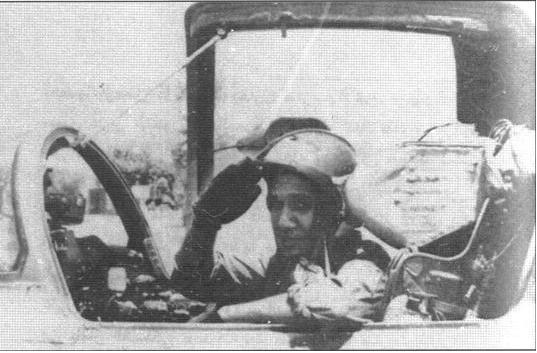
\includegraphics[scale=0.7]{History_Fenix/E3K1MfpzNMk.jpg}
	%	\label{fig:scipion} % Unique label used for referencing the figure in-text\end{document}
	%	%\addcontentsline{toc}{figure}{Figure \ref{fig:placeholder}} % Uncomment to add the figure to the table of contents%----------------------------------------------------------------------------------------
	\caption{Михаиль в кабине МиГ-21. Фото group73historians}%	CHAPTER 2
\end{figure}

Часто пишут, что в том бою обе стороны заявили по одной победе, в то время как в реальности ни одного самолёта сбита не было. Это не совсем верно. Был сбит один МиГ-21 102-й иабр, повреждены один МиГ-21 104-й иабр (того самого Исмаила Имама) и “Мираж” Розена из 119-й эскадрильи. К слову, сначала израильтяне заявили о двух сбитых МиГах - но позже, когда выяснилось что самолет Исмаила Имама дотянул до аэродрома, сократили заявки до одной.

Израильтянин же, поразив МиГ-21 капитана Ахмада Нур Эд-Дина из 102-й авиабригады, решил “досмотреть кино” - проследить траекторию падения самолёта. Эту ошибку совершали десятки летчиков до него и очень многие - после. Для того, чтобы прицелиться и выпустить ракету, египетскому пилоту (которым и был Самир Азиз) хватило нескольких секунд.

Но самое комичное началось уже после возвращения. Вскоре выяснилось, что фотокинопулемет на самолете Самира Азиза не работал, и командиры заставили его писать длинное объяснение - что он делал в бою, что видел - и почему считает, что он сбил “Мираж”. Причина такого дотошности вскрылась быстро - предполагалось, что самолёт 102-й иабр был по-ошибке сбит кем-то из своих.

Что характерно - египтяне скорее были готовы поверить в то, что Самир сбил свой самолет, чем в то, что он сбил “Мираж”. Но это частности. А текущие события подтверждали большие проблемы египтян - 21 мая 69-го “Миражи” всё той же 119-й эскадрильи затянули в ближний маневренный бой и сбили три египетских МиГ-21, все сбиты пушками. Отличились Комэск Ран Ронэн, старший замкомэска Ашер Снир и всё тот-же Реувен Розен. Египтяне подтвердили два сбитых МиГ-21.

Дальше дела у египтян шли не очень здорово — он достигали некоторых успехов в атаках израильских позиций, но потери при этом несли существенные. Что важно — во время налётов на Синае погибли или попали в плен много опытных лётчиков МиГ-17 и Су-7. У истребителей, как правило воевавших над Египтом, было больше шансов покинуть самолёт над своей территорией.

Классикой израильской тактики того времени были засады в воздухе — одна пара выманивает противника, вторая — ждёт на малой высоте, и в нужный момент атакует. Работало часто и почти безотказно — правда, вскоре сами египтяне попытались взять эту тактику на вооружение. Получилось не сразу — но получилось! 

\section{Первая победа}

20 июля 69-го египтянам удалось выманить два израильских “Миража” маневрами демонстративной группы и сбить их фирменной израильской атакой снизу. 

\begin{textcitation}
	"МиГ-17 развернулись в сторону Мансуры, но у меня всё ещё было достаточно топлива и я жаждал боя. Я набрал высоту, чтобы убедиться, что израильские радары видят меня. Мы сделали полный круг, но никто не появился. Тут я увидел четвёрку «Миражей», набирающих высоту и подбирающихся к первому и второму номеру нашего звена, и один за другим выпускающими ракеты. Я довернул на них, и чтобы помочь им, выпустил ракету в сторону ближайшего «Миража» — грубо, без сигнала захвата цели. Случилось чудо — моя ракета поразила цель. Была большая вспышка, и моя цель начала разваливаться на части. Другие израильтяне тут-же отвернули в сторону Синая, а повреждённый самолёт летел за ними. У меня было мало топлива, и я не преследовал его, но разведка после боя подтвердила, что израильский пилот катапультировался, а самолёт упал на другой стороне Канала…"
\end{textcitation}

Что характерно, Михаиль пишет «наши первый и второй номера», как о товарищах по эскдрилье — по другим источникам, лётчики были из 44-й иабр. Их ведущий, майор Хассан Хедр, был сбит несколькими минутами позже — избежав ракет «Миражей», его самолёт не пережил встречи с собственной ПВО.

Израильская сторона подтверждает потерю двух «Миражей» в тот день, правда при несколько иных обстоятельствах. Были сбиты лейтенанты Эли Зоар и Эйтан бен Элияху, будущий главком ВВС Израиля. Иногда пишут, что Зоар был сбит в воздушном бою, а бен Элияху — огнём ПВО. В своё время этот вопрос обсуждался на израильском форуме https://www.fresh.co.il, причём один из участников утверждал, что Бен-Элияху совершенно точно был сбит в воздушном бою, а версия с ПВО появилась позже. Так этот или нет, я не знаю, да и к теме статьи это особо не относится. В случае с Зоаром всё проще — на сайте Амира Сегева пишут, что в его самолёте вышла из строя радиоаппаратура, и пилот не услышал многочисленных предупреждений.

И да, по израильской версии «Миражей» было два. Вероятно, оба до последнего момента были увлечены погоней за МиГами демонстративной группы и не заметили угрозы. Со стороны египтян это было первое успешное применение засадной тактики - и практически последнее. Потеря двух машин в воздушных боях в день была для израильтян очень неприятным эпизодом, и они достаточно быстро выработали меры противодействия. Ну, и сказывалось качество их взаимодействия с наземным КП, куда выше чем у арабов.

\begin{figure}[h!tb] 
	\centering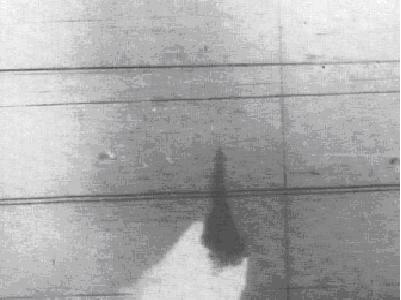
\includegraphics[scale=0.9]{History_Fenix/4syfS9htP7E.jpg}
	%	\label{fig:scipion} % Unique label used for referencing the figure in-text\end{document}
	%	%\addcontentsline{toc}{figure}{Figure \ref{fig:placeholder}} % Uncomment to add the figure to the table of contents%----------------------------------------------------------------------------------------
	\caption{Горящий «Мираж» - часто это фото датируют 20 июля}%	CHAPTER 2
\end{figure}

13 сентября случилось ещё одно большое столкновение. 9 сентября случился знаменитый «Равив» - рейд израильской бронетехники за Канал. 11 сентября египтяне ответили — массированным налётом на израильские позиции ПВО. 46-я иабр в тот день эскортировала МиГ-17, атаковавших израильские ЗРК. Разразился большой воздушный бой (фактически, стычки разного состава продолжались практически с первого налёта — египтяне прилетали, израильтяне перехватывали их и преследовали на пути домой). Самир атаковал один из Миражей (судя по израильскому описанию того боя, им был Одед Мааром из 119-й эскадрильи, увернувшийся от четырёх советских ракет "Атолл».

\begin{textcitation}
	Когда мы возвращались назад в сторону Канала, МиГ-17 были атакованы четвёркой «Миражей». Мы спикировали с высоты в 5 километров, когда израильтяне были заняты тем, что охотились на 17-е, которые крутились на одном месте как могли. Израильтяне не увидели нас, но в той ситуации мы не могли использовать наши ракеты (пушек к МиГ-21 ФЛ не было). Когда израильтяне наконец подобрались достаточно близко, чтобы атаковать 17-е пушками, замыкающий звена МиГ-17 совершил ошибку. В крутом левом повороте он зацепил крылом землю, и его самолёт тут же превратился в огромный огненный шар. Два "Миража» начали набирать высоту, и мы бросились за ними. Я сказал моему второму номеру приготовиться к атаке. Я выпустил обе ракеты и видел их белые хвосты, летящие к цели. Мне казалось, что я не мог промахнуться, но израильский лётчик оказался опытным пилотом, он вошел в крутой вираж, сделал бочку и спикировал вниз. Мы остались без вооружения и вышли из боя. 
\end{textcitation}

Другая пара «Миражей» ввязалась в бой с другой парой 21-х из 26-й эскадрильи, майора Фавзи Салама и лейтенанта Мустафы Гема. Фавзи Салама промахнулся, а его второй номер заявил одну победу. По другой (возможно, непротиворечивой) версии, ещё одну победу записал себе лейтенант Реда Сакр.

В тот день израильтяне заявили 7 сбитых в воздушных боях (5 МиГ-21 и 2 Су-7), и ещё три записали на счет ПВО (один МиГ-21 и два МиГ-17). Египтяне подтверждают потерю 8 машин. Потери Израиля составили один «Мираж» — его пилот, первый израильский ас капитан Гиора Ромм попал в плен. С его слов, его сбили на высоте около 20 000 футов — так что на победу могут претендовать оба египтянина.

В Израиле главной причиной потери самолёта посчитали привычку пилотов «Миражей» размыкать пары в ходе боя - стремясь одержать как можно больше побед, они часто воевали поодиночке.

«МиГи стреляли с любых углов. Их шансы попасть были невелики, но они всё равно стреляли. В учебных боях, когда ты видишь самолёт с такого ракурса, ты игнорируешь его, но в этом конкретном бою египтяне стреляли из любых положений. По мне дважды открывали огонь даже из передней полусферы" — так описывает тот бой один из израильских лётчиков 119-й эскадрильи.

После этого, египтяне прекратили все попытки завоевать превосходство в воздухе, и сконцентрировались на сопровождении собственных ударников «за Канал» и перехвате израильтян.

До конца войны на истощение, Самир Михаиль принял участие в нескольких столкновениях с израильтянами. Он не одержал побед, и не были сбит.

46-я иабр до конца войны потеряла несколько самолётов и сумела одержать ещё одну возможную победу.

В феврале 70-го очередной бой “Миражей” 101-й эскадрильи и МиГ-21 104-й авиабригады закончился со счетом 1:1 - теперь уже арабы подловили израильтянина (за минуту до того сбившего 21-й), когда тот пытался выйти из боя с аварийным остатком топлива. Израильтяне подтверждают потерю одного «Миража» (лётчик, Авиноам Келдес, попал в плен).

Самир Михаиль участвовал в войне, которую в его стране назовут Октябрьской. 8 октября 1973 года он был сбит в воздушном бою с лётчиками 101-й эскадрильи ВВС Израиля. Самир Михаиль исполнял обязанности командира эскадрильи. Победу одержал Эйтан Карми (в тот день он сбил 2 МиГ-21, Самира Михаиля и его ведомого, лейтенанта Салаха). Сам Эйтан Карми также был сбит другим МиГ-21, предположительно пилотируемым номером 3 в звене Михаиля, Абиделем Хаммамом. Тот бой закончился со счетом 3:1. Ещё одну подтвержденную победу одержал резервист и летчик-испытатель проекта "Кфир" Асаф Бин-Нун.

Самиру удалось катапультироваться, он был подобран арабским рыбаком, провел несколько недель в госпитале с компрессионным переломом позвоночника. Его потеря стала тяжелым ударом для эскадрильи. Восстановился на лётной работе. В дальнейшем стал генерал-майором, дал множество интервью. Активно поддерживал президента Мубарака. 

Использованы источники \cite{kuper_nikole,kair_hist,segev,skywar,giora}. Все фотографии взяты с сайта http://group73historians.com

Ссылка на оригинал \url{https://vk.com/wall-162479647_34608}

К оглавлению на странице \pageref{tablecont}